\chapter{Specific Requirements}

\section{External Interface Requirements}
\subsection{User Interfaces}
\subsection{Hardware Interfaces}
This section describes the logical and physical characteristics of each interface 
between the hardware and software componenents of the system.\\
Both educators and students need to have a computer to use the CKB platform.\\
\subsection{Software Interfaces}
This section describes the connections between the system and other specific software components.\\
CodeKataBattle is a web application, so it needs a web browser to be used.\\
\subsection{Communication Interfaces}
This section describes the requirements associated with any communication function required
by this system.\\
All the communications of the eMall infrastructure are made via the HTTP application layer
protocol: obviously, all the devices using the platform must be connected via WiFi or mobile
network (LTE/3G/4G/5G).\\

\section{Functional Requirements}
\subsection{Use Cases Diagrams}
\begin{figure}[H]
    \centering
    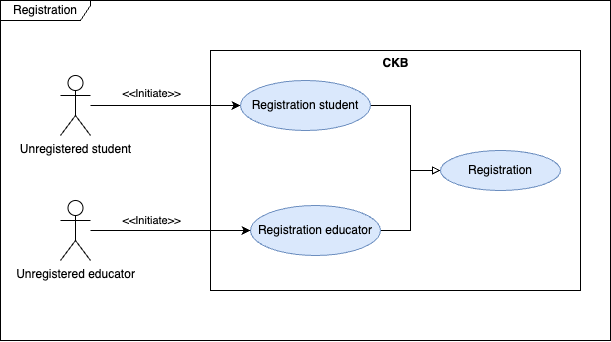
\includegraphics[width=0.8\textwidth]{images/use_cases_diagrams/Registration.png}
    \caption{Unregistered user (student or educator) use case diagram}
    \label{fig:use_case_diagram}
\end{figure}
\clearpage

\subsection{Sequence Diagrams}
\begin{figure}[H]
    \centering
    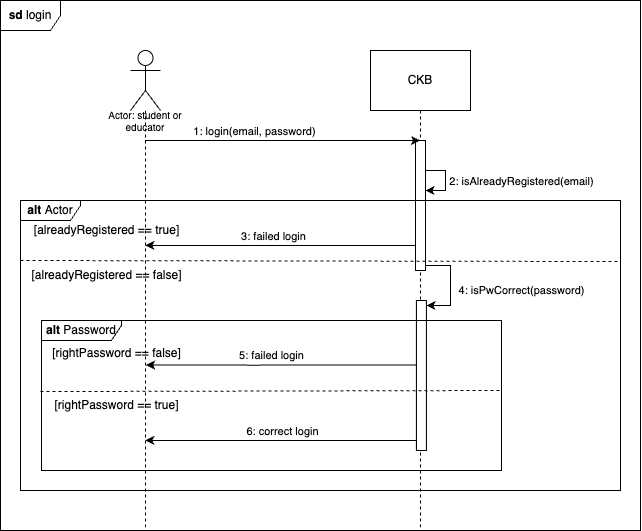
\includegraphics[width=0.9\textwidth]{images/seq_diagrams/Login.png}
    \caption{Login sequence diagram}
    \label{fig:sequence_diagram}
\end{figure}
\clearpage

\section{Performance Requirements}

\section{Design Constraints}
\subsection{Standards compliance}
\subsection{Hardware limitations}
\subsection{Any other constraint}

\section{Software System Atttributes}
\subsection{Reliability}
\subsection{Availability}
\subsection{Security}
\subsection{Maintainability}
\subsection{Portability}

